\chapter{Evaluation} \label{ch:evaluation}

In this chapter, we implement FHS and GES into a centralized wireless resource
scheduling problem with underlying GE channel and evaluate the behavior as well
as the performance of our proposed method in simulations. To provide an
appropriate comparison, in Sec.~\ref{sec:setup} we describe our choices for the
simulation environment and introduce three testing scenarios with different
network configurations. Finally, we present and discuss the results of different
simulations in Sec.~\ref{sec:results}. 

\section{Simulation Setup} \label{sec:setup}
% Details regarding implementation and/or simulation are given in this chapter.
% The considered setup and the parameters used are introduced and discussed. Also,
% the general evaluation methods can be presented. (Note: Code should not be part
% of this chapter. If it makes sense to introduce it into the thesis, it should be
% placed in the appendix.)

Suppose a minimal simulation environment comprising of $N=3$ control sub-systems
sharing a GE wireless channel to demonstrate the benefit of finite horizon
minimization. In order to provide intuitive and illustrative results, we
consider scalar sub-systems in the evaluation. Each sub-system is chosen to have
different plant system dynamics, with increasing unstable system matrices, i.e.,
$A_{1,2,3} = \left\{1.0, 1.25, 1.5\right\}$. The input matrix is given by $B_i =
1.0, \forall i$. The control sub-systems are initialized with $x_i[0] = w_i[0]$
for all $i$ and system noise is characterized by $w_i[k]\sim \mathcal{N}(0,1)$,
i.e., $\Sigma_i=1$. Among the simulated sub-systems, $A_3=1.5$ represents the
most challenging application, as its system state evolves the most within a
control time step $k$. Moreover, sub-systems are sampled periodically every 3
slots, i.e., $D_i=3$. To enable non-synchronized sampling, we determine the
initial sampling event randomly from a discrete uniform distribution as $t_{i,o}
= \mathcal{U}\{0, D_i-1\}$. \\
The control law is selected with respect to $\boldsymbol{Q}_i = 1$ and
$\boldsymbol{R}_i = 1$. That is, we solely account for state cost and allow
arbitrary control inputs. According to Eq.~\eqref{eq:optimalgain}, the optimal
feedback gain matrix is determined as $\boldsymbol{L}^*_i = A_i$, which
corresponds to deadbeat control strategy. 

\begin{table}[htb]
  \begin{center}
  \begin{tabular}{|lc|c|c|c|} 
  \hline
  \multicolumn{2}{|c|}{\textbf{Channel model parameters}} & \textbf{Scenario 1} & \textbf{Scenario 2} & \textbf{Scenario 3} \\
  \hline \hline
  Loss in Good & $p_G$ & 0.25 & 0.25 & 0.0011 \\ 
  Loss in Bad & $p_B$ & 0.75 & 0.75 &  0.7734 \\ 
  Failure rate & $f$ & 0.3 & 0.1 & 0.0024 \\ 
  Recovery rate & $r$ & 0.3 & 0.1 & 0.0832 \\
  \hline
  Average error probability & $p_E$ & 0.5 & 0.5 & 0.0227 \\
  Mean sojourn time in Good & $T_G$ & 3.33 & 10 & 416.66 \\
  Mean sojourn time in Bad & $T_B$ & 3.33 & 10 & 12 \\
  \hline
  \end{tabular}
  \end{center}
  \caption{Summary of evaluation scenarios and their Gilbert-Elliot channel parametrization}
  \label{tab:scenarios}
\end{table}

Table~\ref{tab:scenarios} depicts the 3 chosen scenarios and their respective GE
channel parametrization. Scenario 1 and 2 resemble challenging GE channels,
where on average half of the packets transmitted are lost. Further, due to
symmetrical state transition probabilities, the channel will be in good and bad
states 50\% of the simulation time on average each. $f$ and $r$ merely differ in
absolute values, making the second channel prone to longer burst errors. To
evaluate scheduler performance in a real-life scenario, we have adopted the GE
parameters for scenario 3 from experiments conducted in
\cite{frohn2011analyzing}. Here, measurements are obtained from an indoor
wireless testbed based on the IEEE 802.11n standard. Obtained network trace is
then used to find analytical GE parameters using the \textit{Baum-Welch
algorithm} \cite{baum1970maximization}. Compared to the first two settings,
scenario 3 provides a good channel with significantly lower average loss
probabilities and stays in the good state for the majority of time. \\ 
For each scenario we vary the finite Horizon $H=\left\{ 1, \cdots, 10\right\}$
for FHS and $H=\left\{ 1, \cdots, 4\right\}$ for GES to study its effect on AoI
and MSE. Each configuration is simulated for a duration of $D=20000$ time slots
and repeated $R=200$ times.

\subsection{Performance Metrics} 

We evaluate scheduling performance in terms of the following metrics. In every
simulation, the average mean squared error of a sub-system $i$ at each slot is
measured as:

\begin{equation*}
  MSE_i = \dfrac{1}{D} \sum_{t=1}^{D}{(\boldsymbol{e}_i(t))^T \boldsymbol{e}_i(t)},
\end{equation*}

where $\boldsymbol{e}_i(t)$ is the estimation error defined in
Eq.~\eqref{eq:estimationerror}. In addition, we analyze the average MSE in the
network given by:

\begin{equation*}
  \overline{MSE} = \dfrac{1}{N} \sum_{i=1}^{N}{MSE_i}
\end{equation*}

MSE indicates the deviation of the estimated state from its true state, thus
quantifying estimation accuracy of estimator $\estimator$ as well as the
uncertainty in the controlled process. In the same fashion, we measure
information staleness at $\estimator$ by means of individual and total average
AoI as follows:

\begin{align*}
  \Delta_i &= \dfrac{1}{D} \sum_{t=1}^{D}{\Delta_i(t)}, \\
  \overline{\Delta} &= \dfrac{1}{N} \sum_{i=1}^{N}{\Delta_i}
\end{align*}

\section{Results and Discussion} \label{sec:results}
% Results of the performed investigations are presented here. Interpretations for
% the observed effects are given and the impact of investigations is discussed. 

\subsection{Age-of-Information Performance}

\begin{figure}[htb]
  \centering
  \begin{subfigure}{0.49\textwidth}
    \centering
    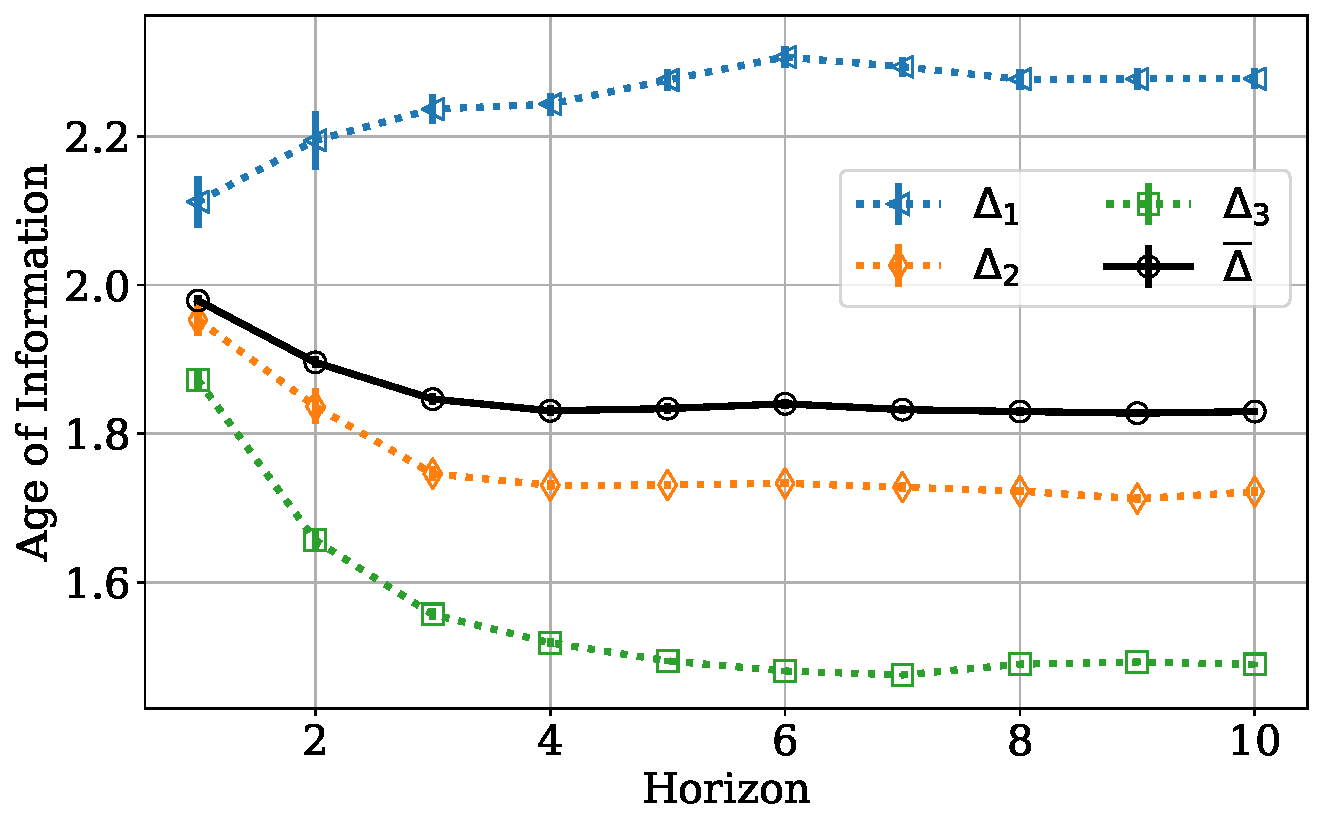
\includegraphics[width=\textwidth]{FHS1_AoI_against_H_separate}
    \caption{Scenario 1 with FHS}
  \end{subfigure}
  \hfill
  \begin{subfigure}{0.49\textwidth}
    \centering
    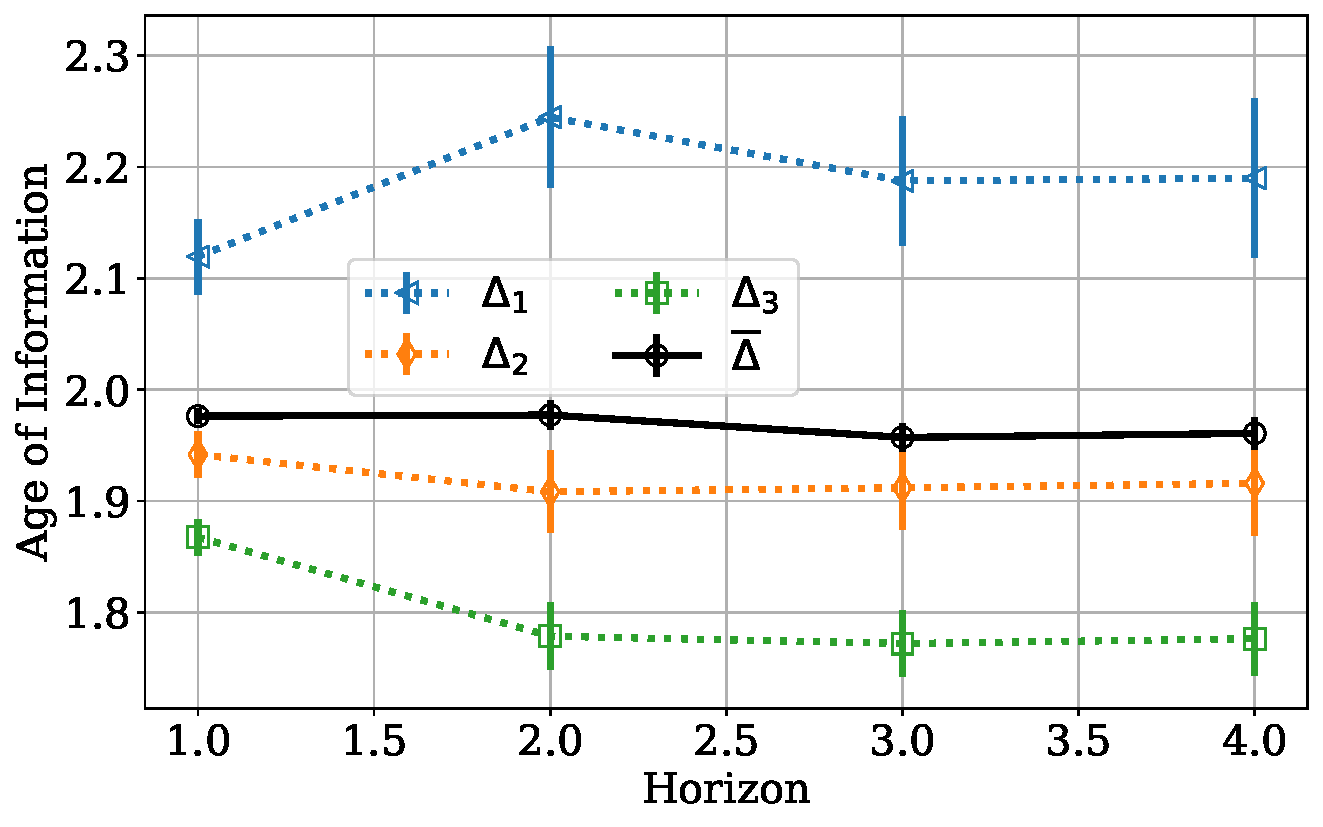
\includegraphics[width=\textwidth]{GES1_AoI_against_H_separate}
    \caption{Scenario 1 with GES}
  \end{subfigure}
\caption[Scenario 1: Average AoI vs. finite horizon $H$]{Achieved average AoI
vs. finite horizon $H$ for FHS and GES. Solid lines $\overline{\Delta}$
illustrate the average AoI in the network per time slot. Dashed lines
$\Delta_1$, $\Delta_2$ and $\Delta_3$ show the average AoI per time slot of each
class with $A_1 = 1.0$, $A_2=1.25$ and $A_3=1.5$, respectively. Vertical bars
represent $95\%$ confidence intervals for $R=200$ simulation runs.}
\label{fig:AoIseperate}
\end{figure}

Fig.~\ref{fig:AoIseperate} depicts the resulting AoI performance among
sub-systems sharing the network for scenario 1. We observe that the average AoI
differs for each sub-system. This is an expected result, since FHS and GES aim
to minimize the short-term MSE trajectory, regardless on how often a loop is
granted medium access. This behavior can be elaborated with the help of
Fig.~\ref{fig:networkshare} which illustrates average network shares of
individual sub-systems. It directly reflects the scheduling decisions taken by
our proposed algorithm. We can examine that the scheduler grants more medium
access to sub-systems, which are expected to produce higher costs. In
particular, we can see that the most critical sub-system $A_3 = 1.5$ is
scheduled in average more frequently. This leads to unequal distribution of
network resource, prioritizing control application the scheduler deems for more
expensive in terms of cost. We further observe that average AoI is inversely
proportional to network share. This make sense since in our scenario, a lower
AoI indicates a more frequent update rate. 

\begin{figure}[p]
\centering
\begin{subfigure}{0.49\textwidth}
  \centering
  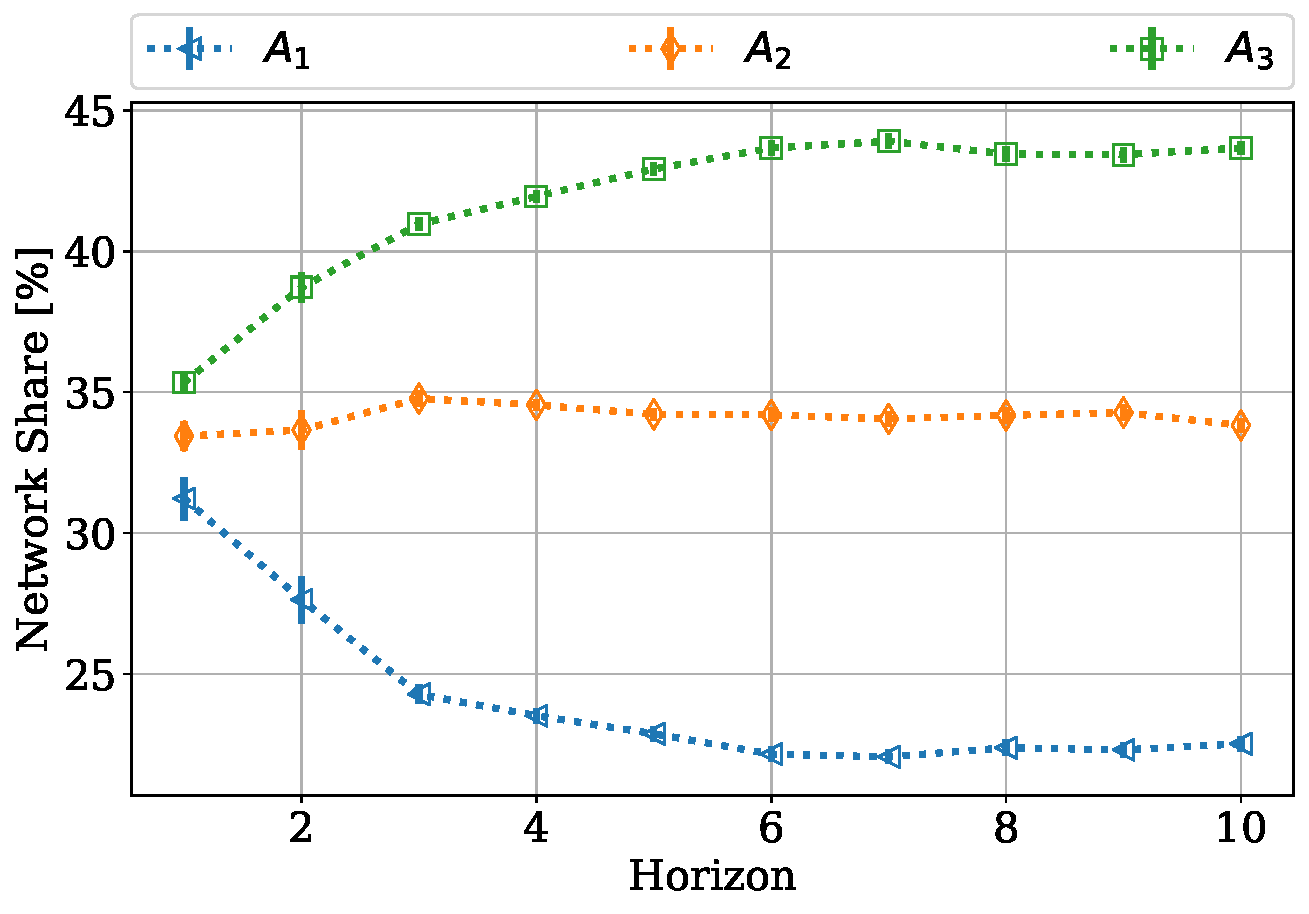
\includegraphics[width=\textwidth]{FHS1_NS_against_H_separate}
  \caption{Scenario 1 with FHS}
\end{subfigure}
\hfill
\begin{subfigure}{0.49\textwidth}
  \centering
  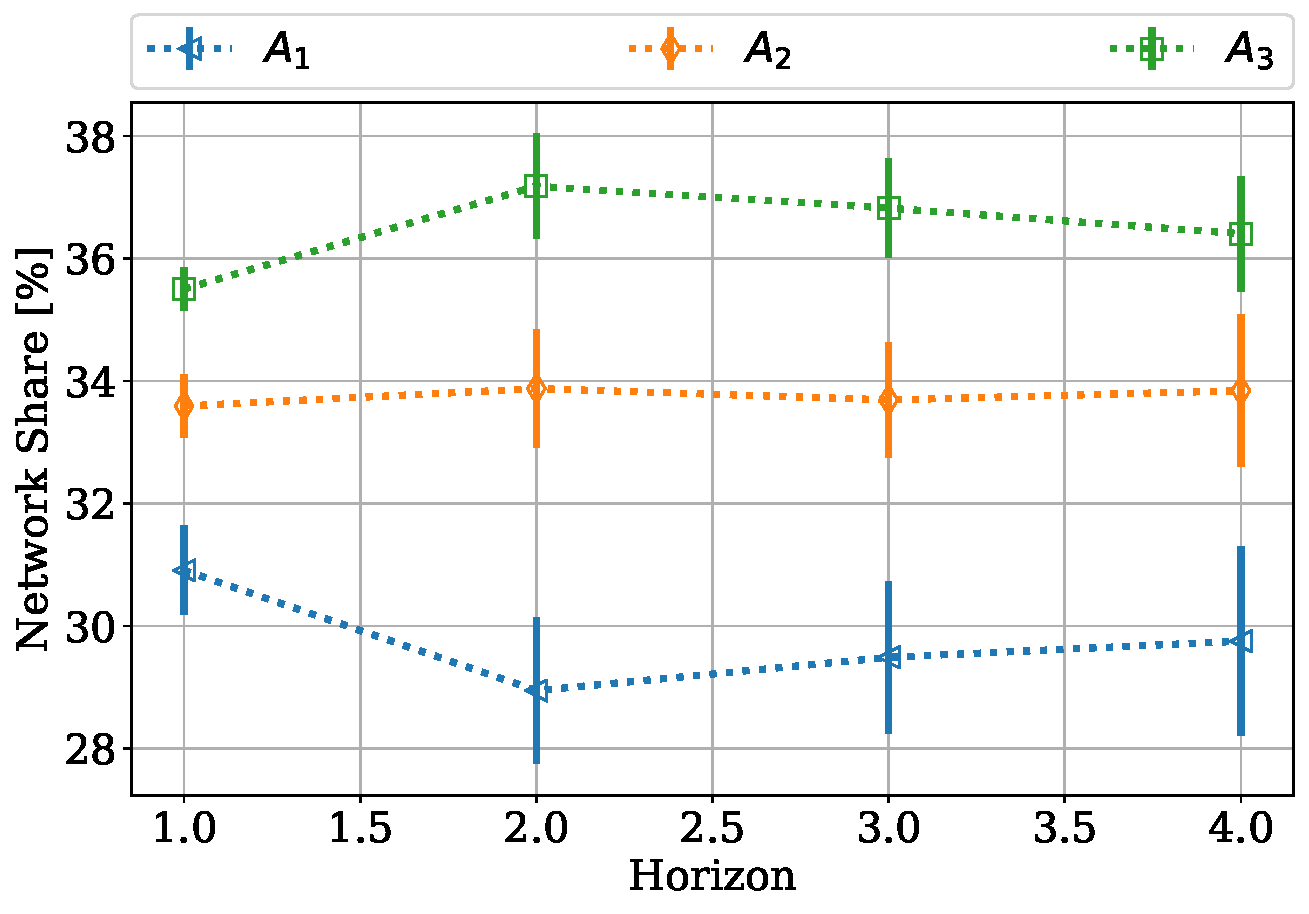
\includegraphics[width=\textwidth]{GES1_NS_against_H_separate}
  \caption{Scenario 1 with GES}
\end{subfigure}
  \caption[Scenario 1: Network share among heterogenous subsystems vs. finite
  horizon $H$]{Network share among simulated sub-systems vs. finite horizon $H$
  over $R=200$ simulation runs. Out of three control loops, only one sub-system
  is allowed to transmit simultaneously. A network share $\alpha_i\%$ indicates
  that the $i$-th sub-system was granted channel access $\alpha_i\%$ of the time
  in average.} 
  \label{fig:networkshare}
\end{figure}

\begin{figure}[p]
  \centering
  \begin{subfigure}{0.49\textwidth}
    \centering
    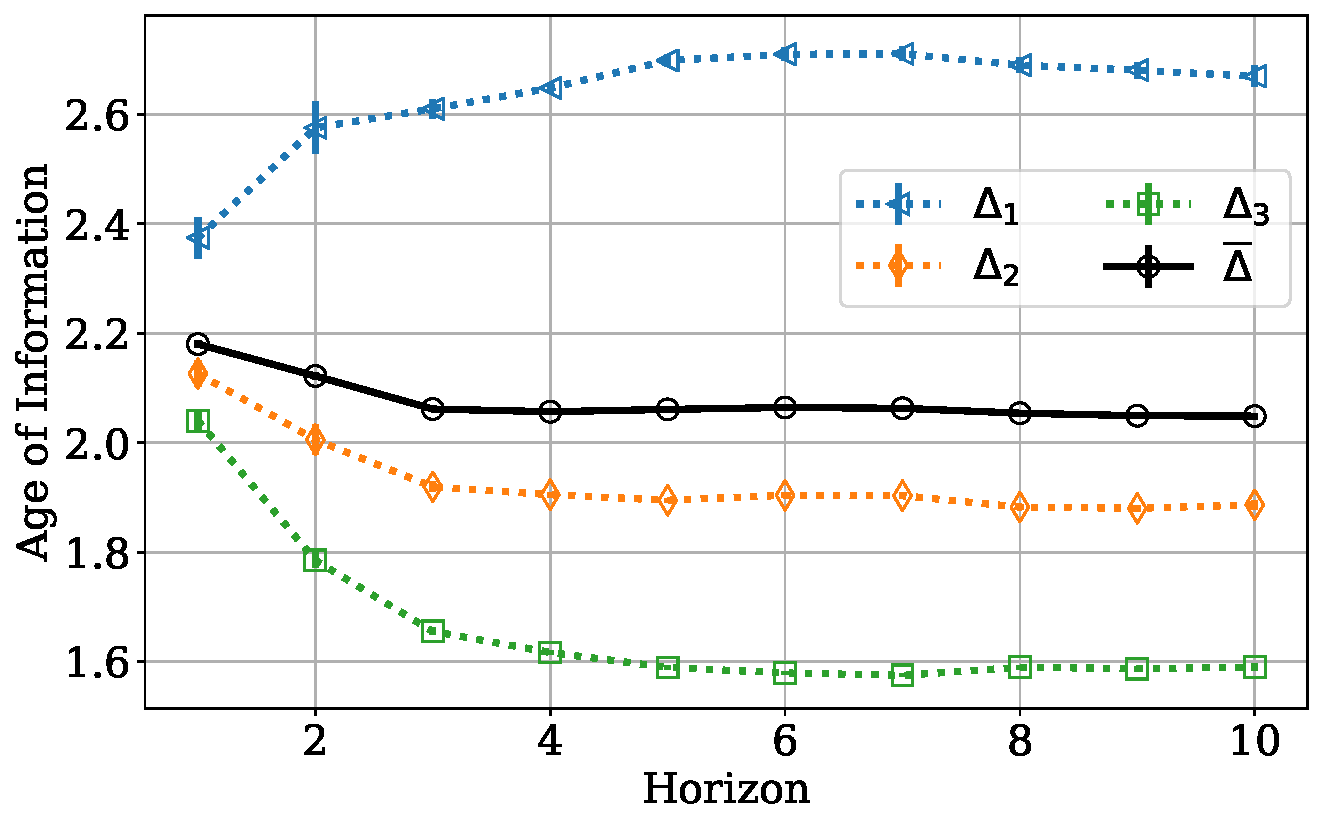
\includegraphics[width=\textwidth]{FHS2_AoI_against_H_separate}
    \caption{Scenario 2 with FHS}
  \end{subfigure}
  \hfill
  \begin{subfigure}{0.49\textwidth}
    \centering
    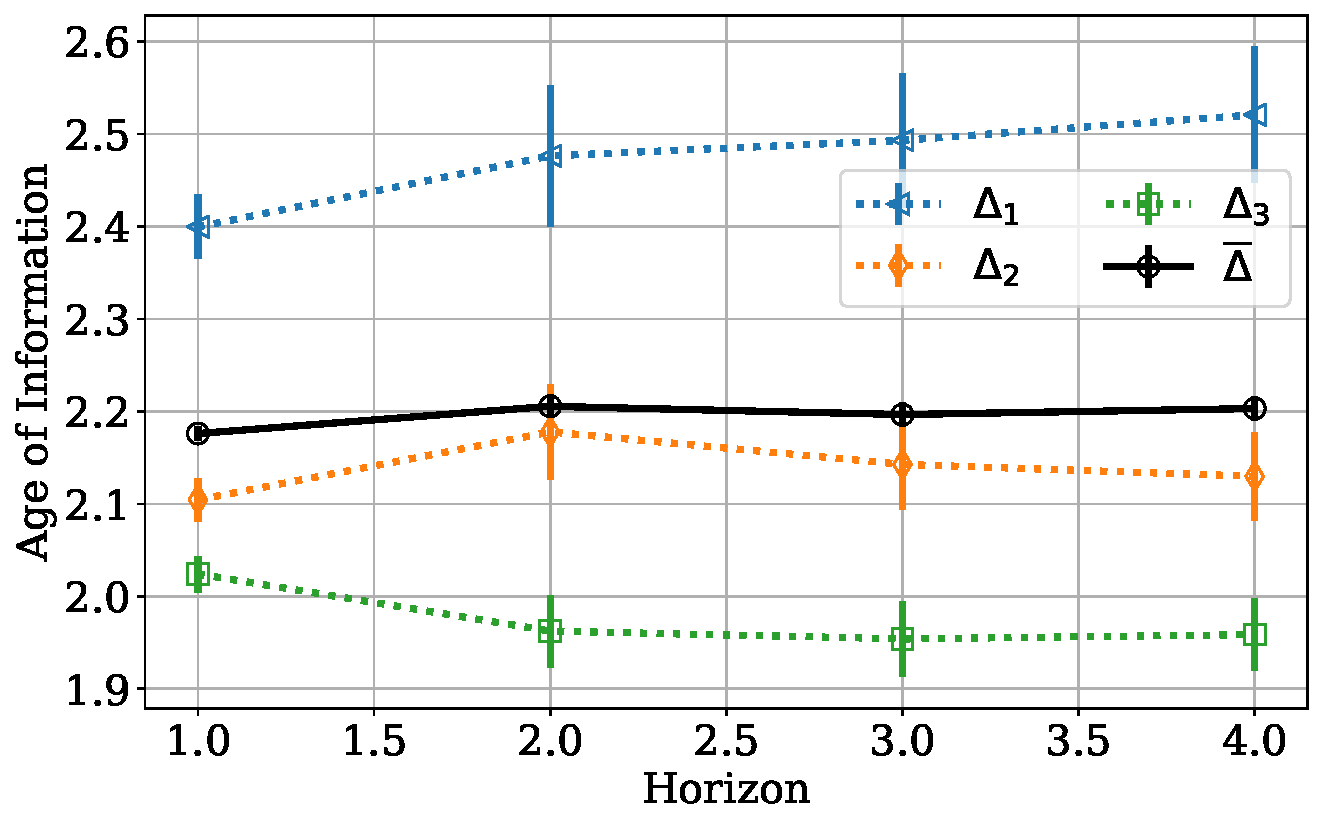
\includegraphics[width=\textwidth]{GES2_AoI_against_H_separate}
    \caption{Scenario 2 with GES}
  \end{subfigure}
  \begin{subfigure}{0.49\textwidth}
    \centering
    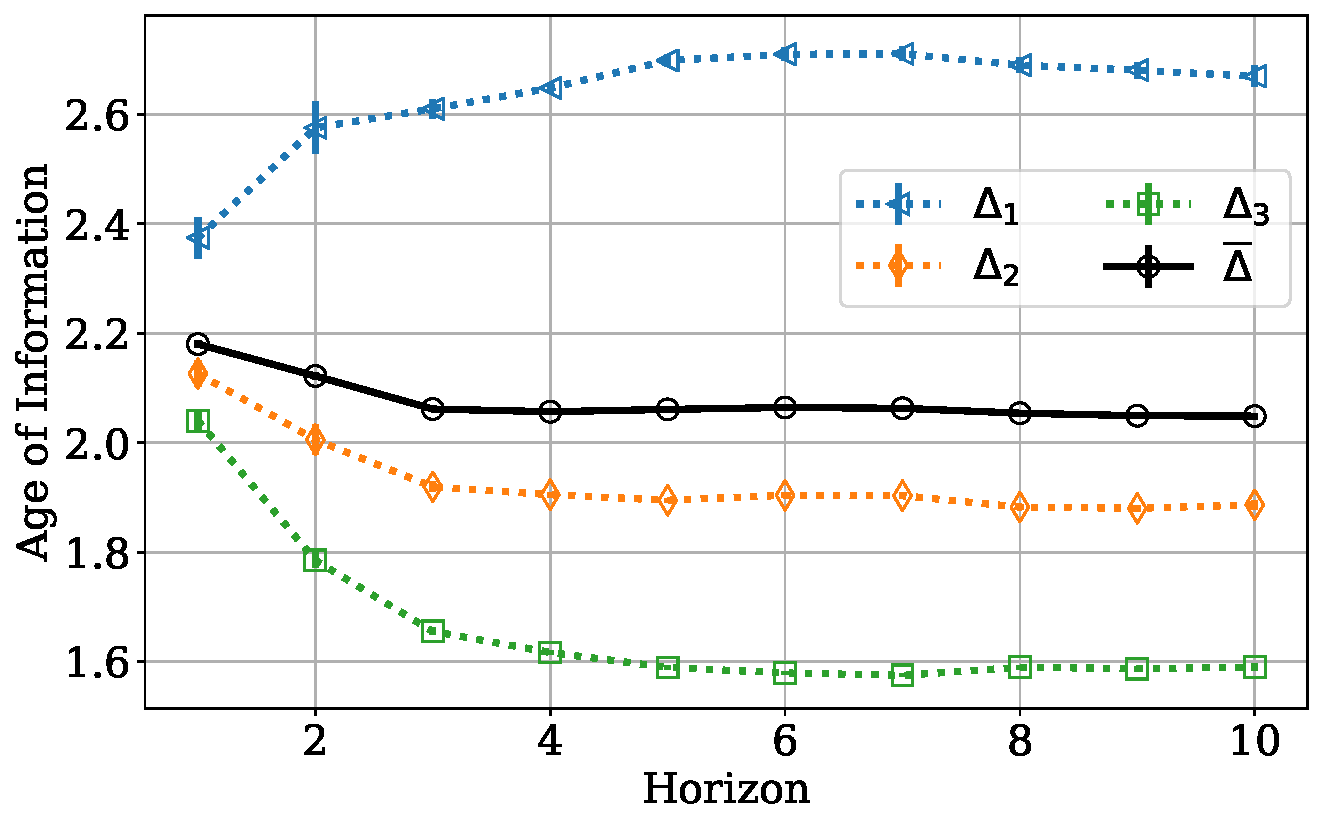
\includegraphics[width=\textwidth]{FHS2_AoI_against_H_separate}
    \caption{Scenario 3 with FHS}
  \end{subfigure}
  \hfill
  \begin{subfigure}{0.49\textwidth}
    \centering
    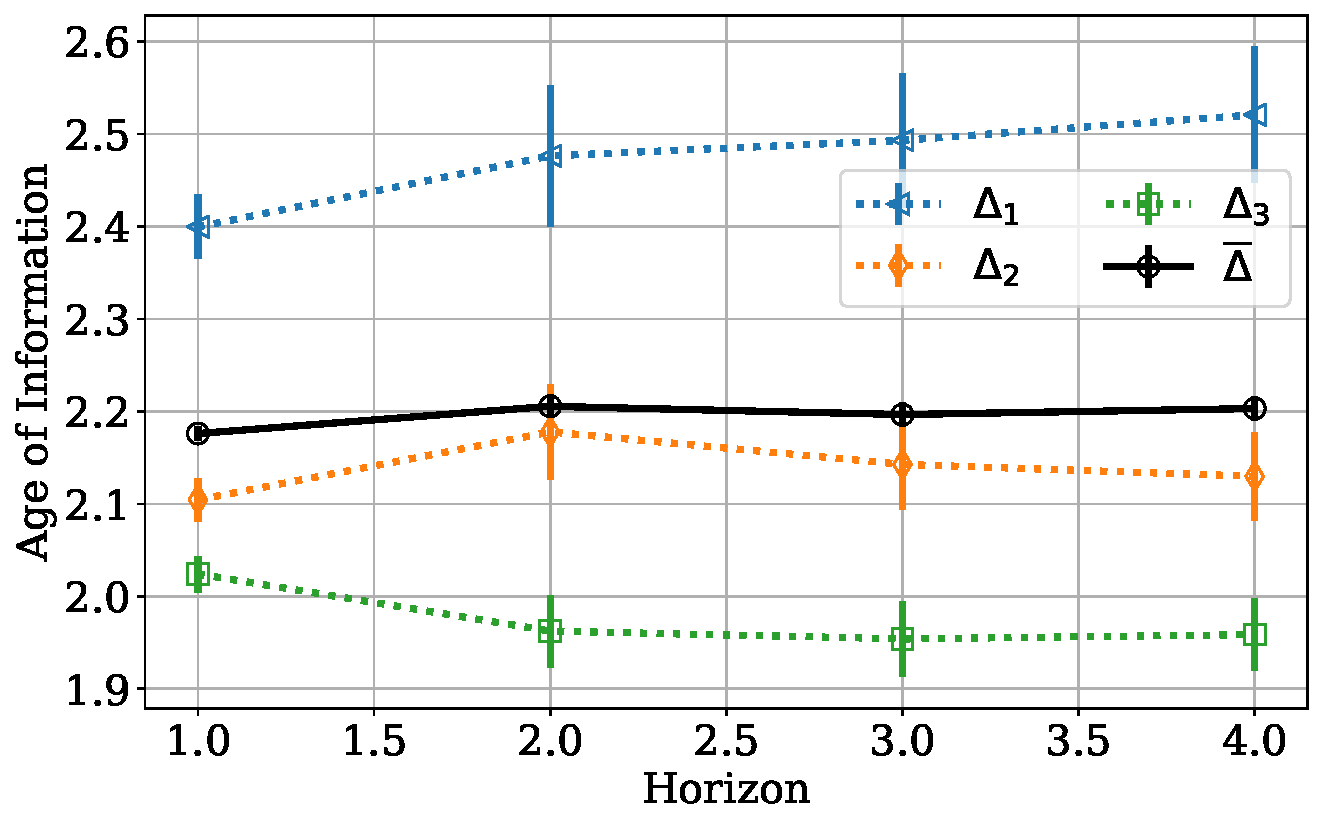
\includegraphics[width=\textwidth]{GES2_AoI_against_H_separate}
    \caption{Scenario 3 with GES}
  \end{subfigure}
  \caption{Scenario 2 \& 3: Average AoI vs. finite horizon $H$}
  \label{fig:AoIseperate2}
\end{figure}

In addition, for FHS we observe a falling trend in $\Delta_2$ and $\Delta_3$ as
$H$ increases. This effect results from the increasing foresight of the
scheduler for possible high future costs in case of consecutive unsuccessful
transmissions. In contrast, GES seems to equalize resource distribution among
sub-systems starting from $H=3$. We interpret this as a result of GES
considering possible GE channel state transitions, while FHS simply assumes the
links to be constant for the next $H$ time slots. For instance, the high cost of
not updating sub-system $A_3=1.5$ is compensated through a high probability of
its link transiting to good state.

Fig.~\ref{fig:AoIseperate2} plots AoI performance for scenario 2 and 3,
respectively. For FHS the same characteristic trend for AoI can be observed.
However, absolute AoI values are shifted upwards for scenario 2 and downwards
for scenario 3. This is a result of different channel quality in each scenario.
Although the average packet loss probability is equal for scenario 1 and 2, the
second channel is expected to stay longer in bad state. This results in longer
consecutive packet losses, thus increasing AoI in the network. The effect on
scenario 3 can be explained analogously.

\subsection{Age-of-Information Distribution}

\begin{figure}[htb]
  \centering
  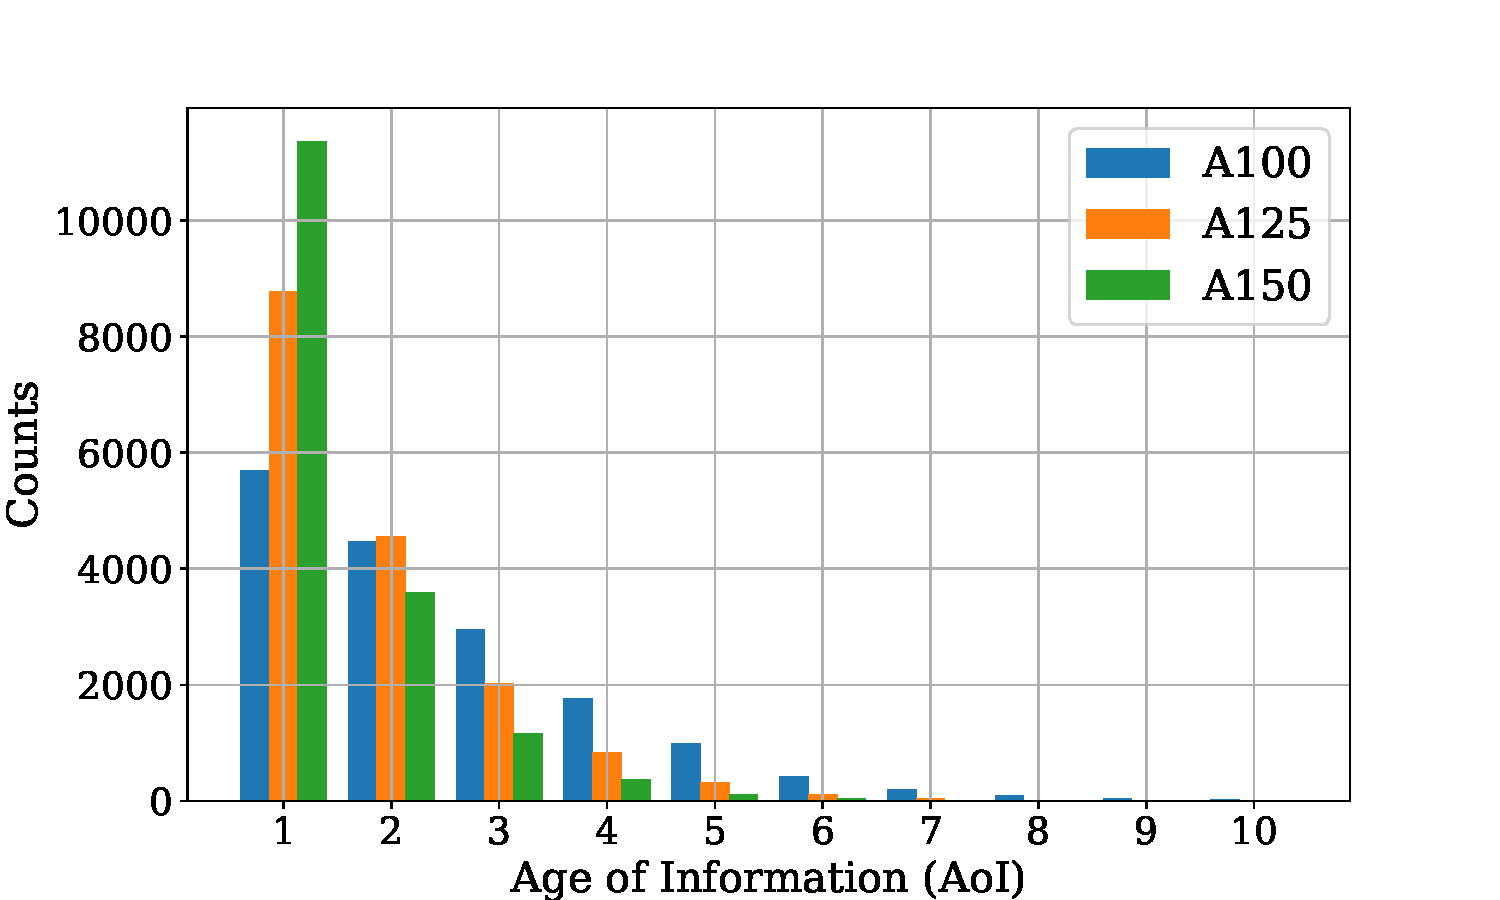
\includegraphics[width=0.6\textwidth]{AoI_Histogram_N3}
  \caption[Scenario 1: Measurement of AoI distribution]{Histogram of perceived
  AoI at controller $\controller$ for simulated sub-systems $A_i=\left\{1.0,
  1.25, 1.5\right\}$ with channel parameters according to Scenario 1. Network
  resources are managed by FHS with $H=2$.} 
  \label{fig:AoIHist}
\end{figure}

Merely examining expected AoI might be misleading and not sufficient when it
comes to time-critical-requirements of underlying sub-systems
\cite{ayan2020probability}. To have a deeper insight of age dependent
performance, we have exemplary measured AoI distribution in the network for one
simulation run consisting of $R=50000$ time slots in scenario 1.
Fig.~\ref{fig:AoIHist} shows the amount of time slots each sub-system were in
the state of respective AoI for scenario 1 and FHS with $H=2$. As expected, the
most up-to-date plant measurements were available to task-critical sub-systems.
This is seen in $A_3$ having the highest AoI=1 count, followed by $A_2$ and
$A_1$. We can see the consequence of the scheduler distributing network
resources unequal, in a shift of counts for higher AoI values. 
  
\cite{ayan2020probability} provides a closed-form expression for the AoI
probability mass function in single and multi-hop networks. In contrast, they
consider a single NCS transmitting over a multi-hop network with time-invariant
packet oss probabilities. Although not directly applicable, we observe a similar
geometric AoI distribution in our measurement. Fig.~\ref{adx:aoiHist} includes
the AoI histogram for the equivalent scenario studied in the paper and validates
their analytical AoI probability mass function for single hop networks.

\subsection{Remote Estimation Performance}

\begin{figure}[htb]
  \centering
  \begin{subfigure}{0.49\textwidth}
    \centering
    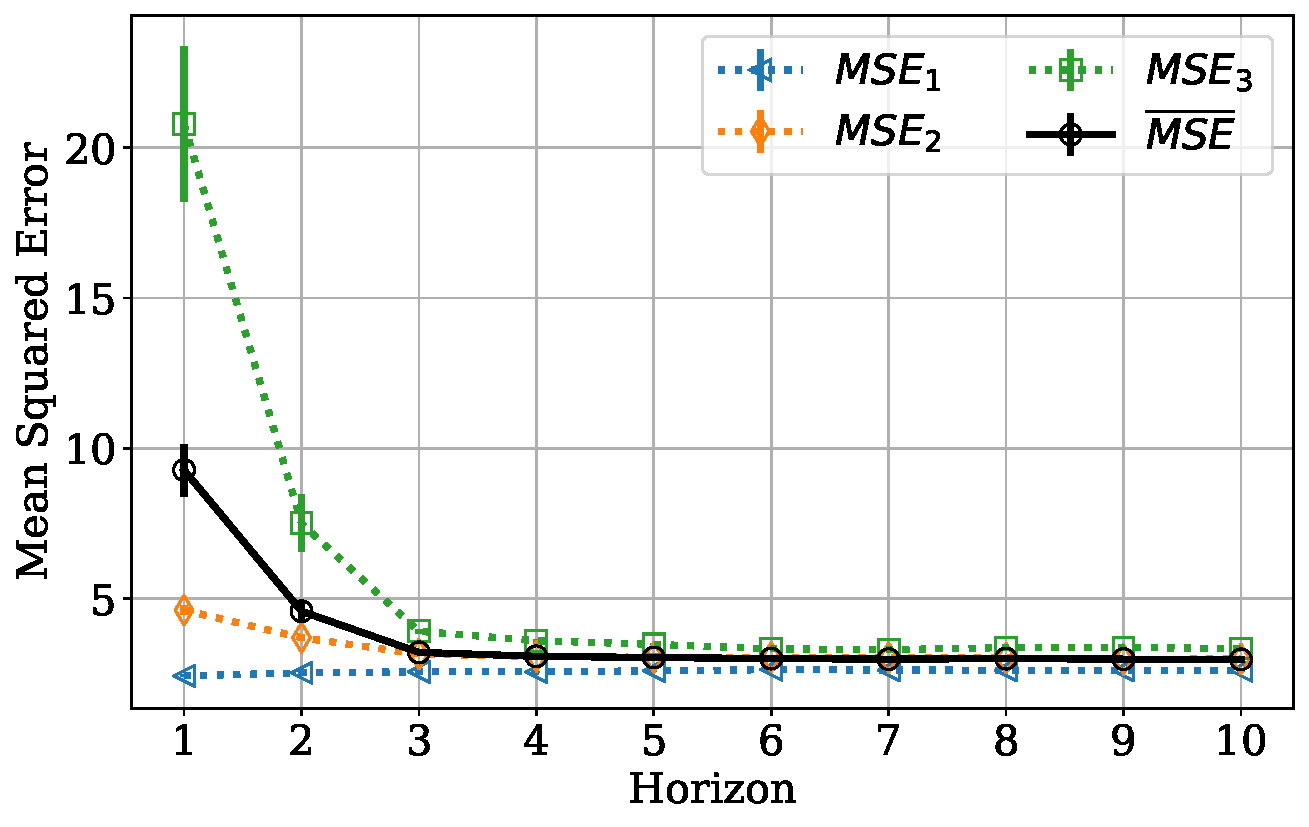
\includegraphics[width=\textwidth]{FHS1_MSE_against_H_separate}
    \caption{Scenario 1 with FHS}
    \label{fig:surprise}
  \end{subfigure}
  \hfill
  \begin{subfigure}{0.5\textwidth}
    \centering
    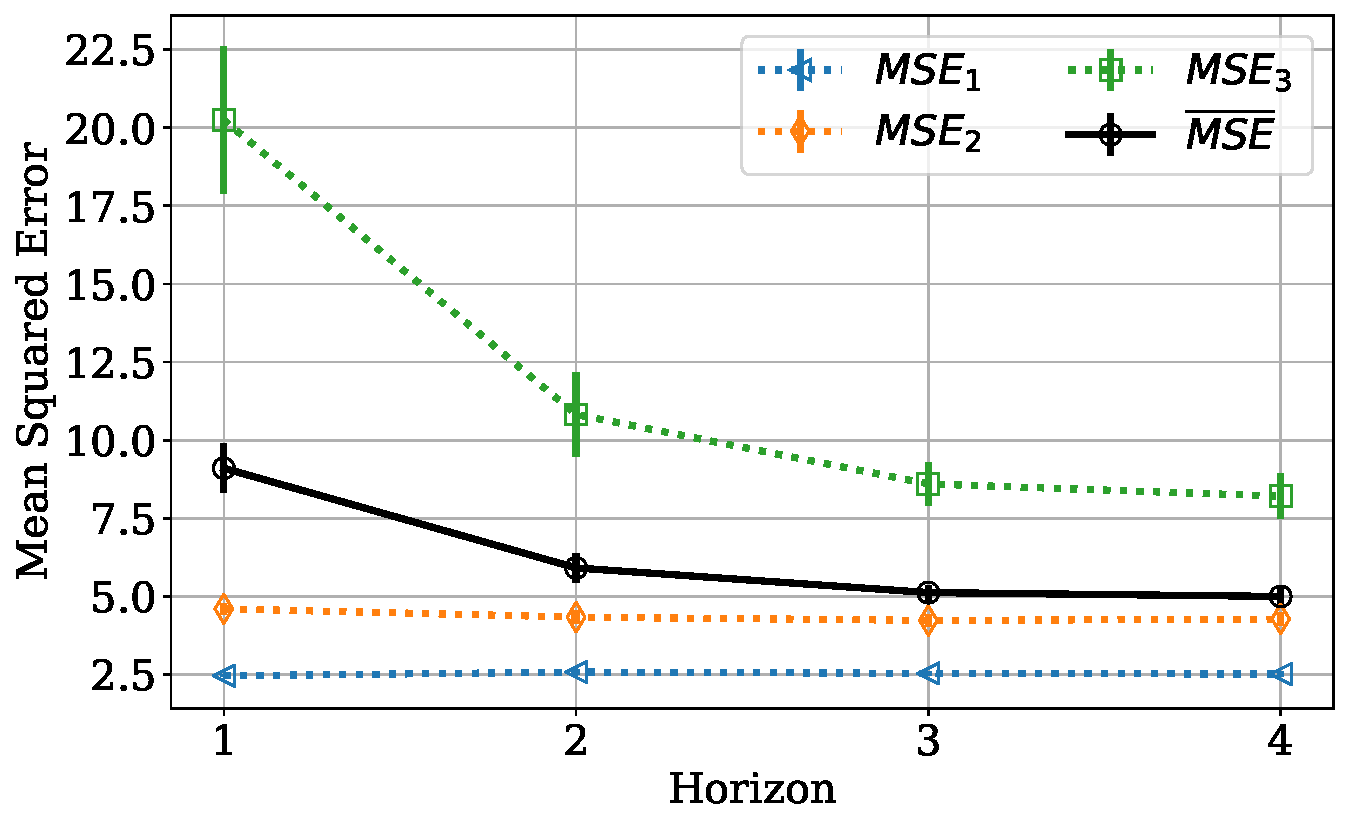
\includegraphics[width=\textwidth]{GES1_MSE_against_H_separate}
    \caption{Scenario 1 with GES}
  \end{subfigure}
  \caption[Scenario 1: Average MSE vs. finite horizon $H$]{Achieved average
  MSE vs. finite horizon $H$ for FHS and GES. Solid lines $\overline{MSE}$
  illustrate the average MSE in the network per time slot. Dashed lines
  $MSE_1$, $MSE_2$ and $MSE_3$ show the average MSE per time slot of each
  class with $A_1=1.0$, $A_2=1.25$ and $A_3=1.5$, respectively. Vertical bars
  represent $95\%$ confidence intervals for $R=200$ simulation runs.}
  \label{fig:MSEavg}
\end{figure}

Putting all our insights of the previous subsections together, we next focus on
our main performance metric $MSE_i$. Fig.~\ref{fig:MSEavg} depicts the
estimation performance achieved by FHS and GES in scenario 1 for varying $H$.
For both FHS and GES, a significant reduction of $\overline{MSE}$ can be seen as
we increase the horizon from $H=1$ to $H=2$. However, beyond $H=2$, as the
scheduler gets more farsighted, the performance gain diminishes and the MSE
trajectory converges. We further examine our scheduler's long-term behavior. As
$H$ increases, the $MSE_i$ lines tend to meet. This effect result from equal
weighing of individual sub-system MSE when obtaining the network cost defined in
Eq.~\eqref{eq:gfunction}. This in turn leads to equal long-term averages as the
scheduling decisions become more ``long-term optimal''. Moreover, notice how
sub-system 3 is the one with the highest MSE in the network, although $\Delta_3$
is the lowest among all $\Delta_i$. This is because according to
Eq.~\ref{eq:estimationerror} estimation error is obtained through AoI and the
underlying system dynamics, meaning that estimation errors propagate differently
for every sub-system.

To our surprise, a slight increase of average MSE in Fig.~\ref{fig:surprise} is
not seen. In a channel with mean sojourn time of 3.33, we initially expected to
observe an increase starting from $H=4$ as the scheduler plans too many time
slots ahead, which would result in possible bad schedules taken in terms of
estimation performance.

Fig.~\ref{fig:MSEavg2} plots FHS and GES estimation performance for scenario 2
and 3. We examine a similar shift for MSE trajectories with FHS due to changing
channel quality. However, in the case of GES, 

% TODO: Add observations for MSEavg2

\begin{figure}[htb]
  \centering
  \begin{subfigure}[b]{0.49\textwidth}
    \centering
    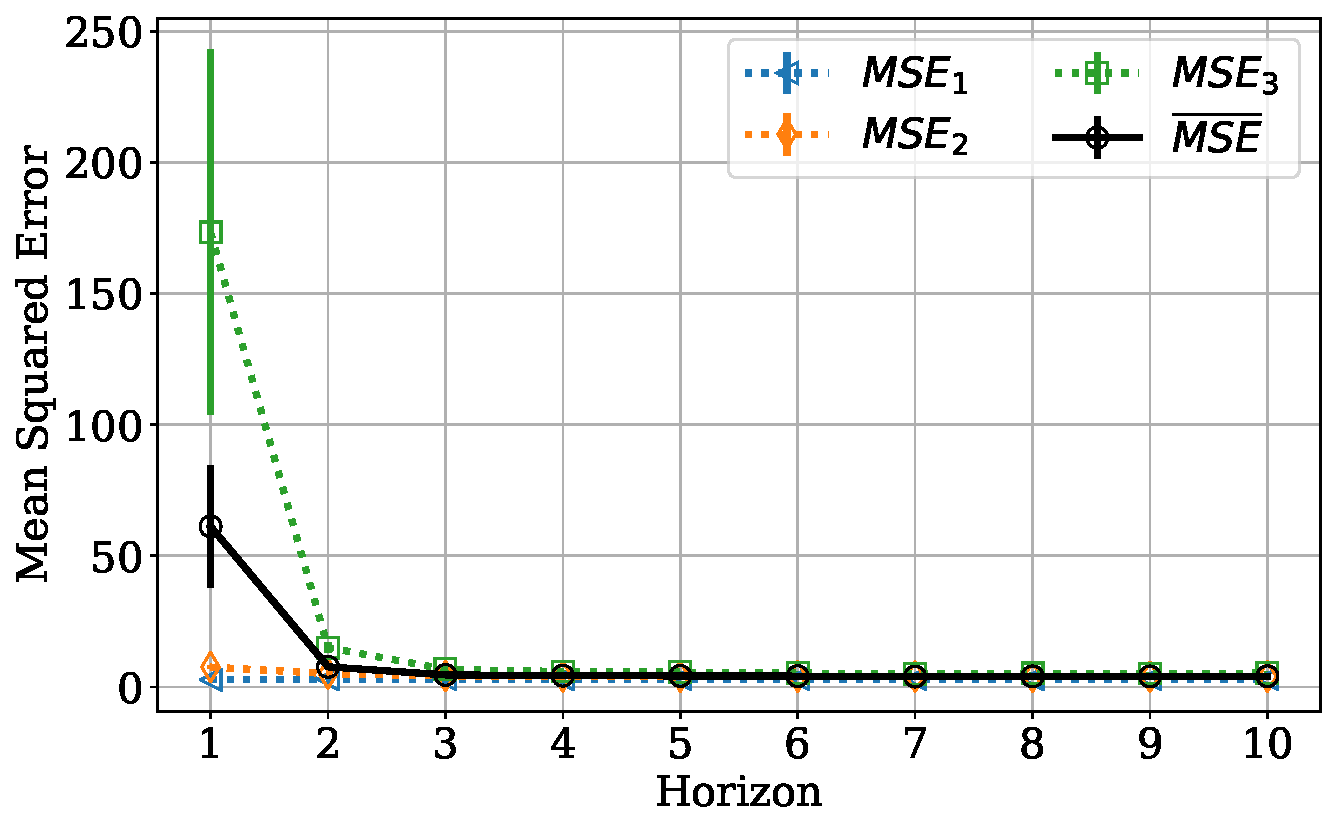
\includegraphics[width=\textwidth]{FHS2_MSE_against_H_separate}
    \caption{Scenario 2 with FHS}
  \end{subfigure}
  \hfill
  \begin{subfigure}[b]{0.49\textwidth}
    \centering
    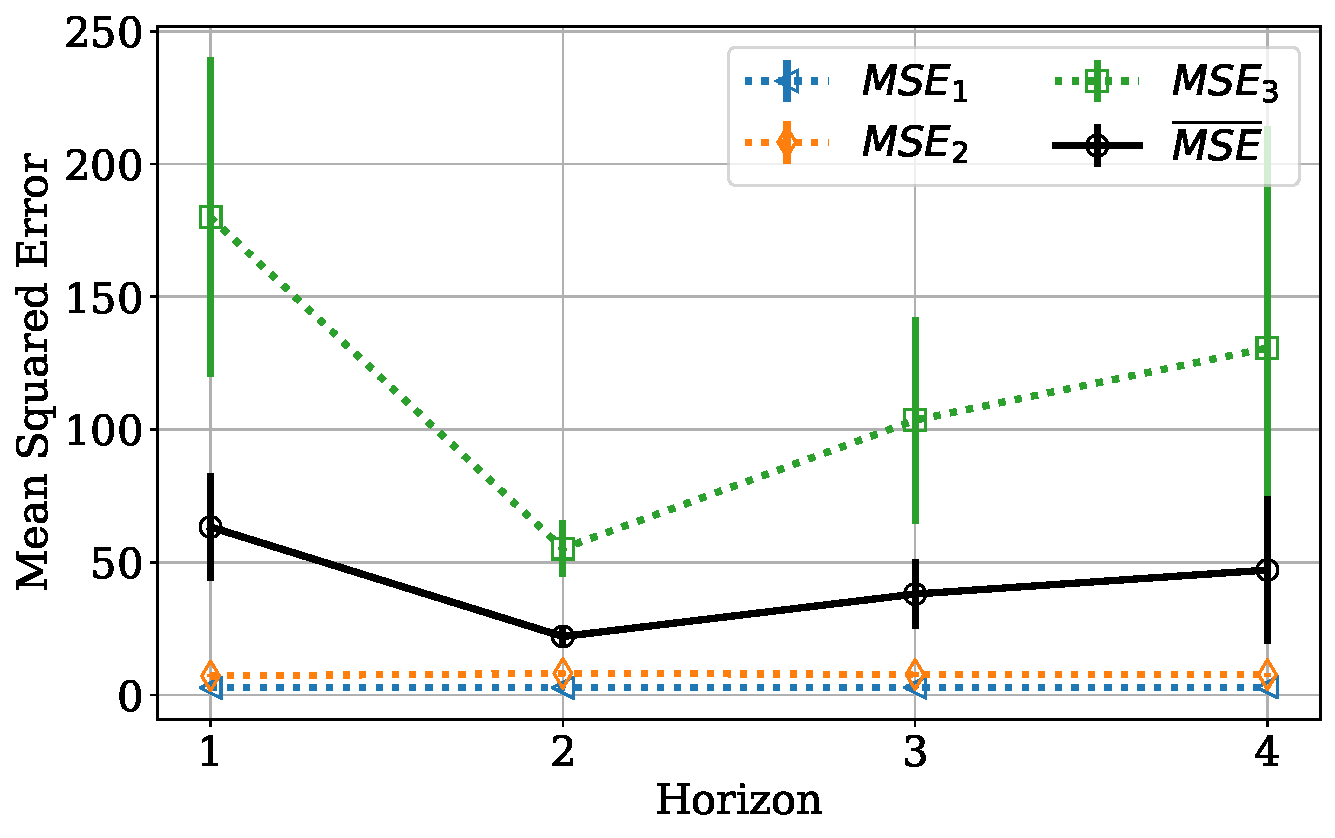
\includegraphics[width=\textwidth]{GES2_MSE_against_H_separate}
    \caption{Scenario 2 with GES}
  \end{subfigure}
  \begin{subfigure}[b]{0.49\textwidth}
    \centering
    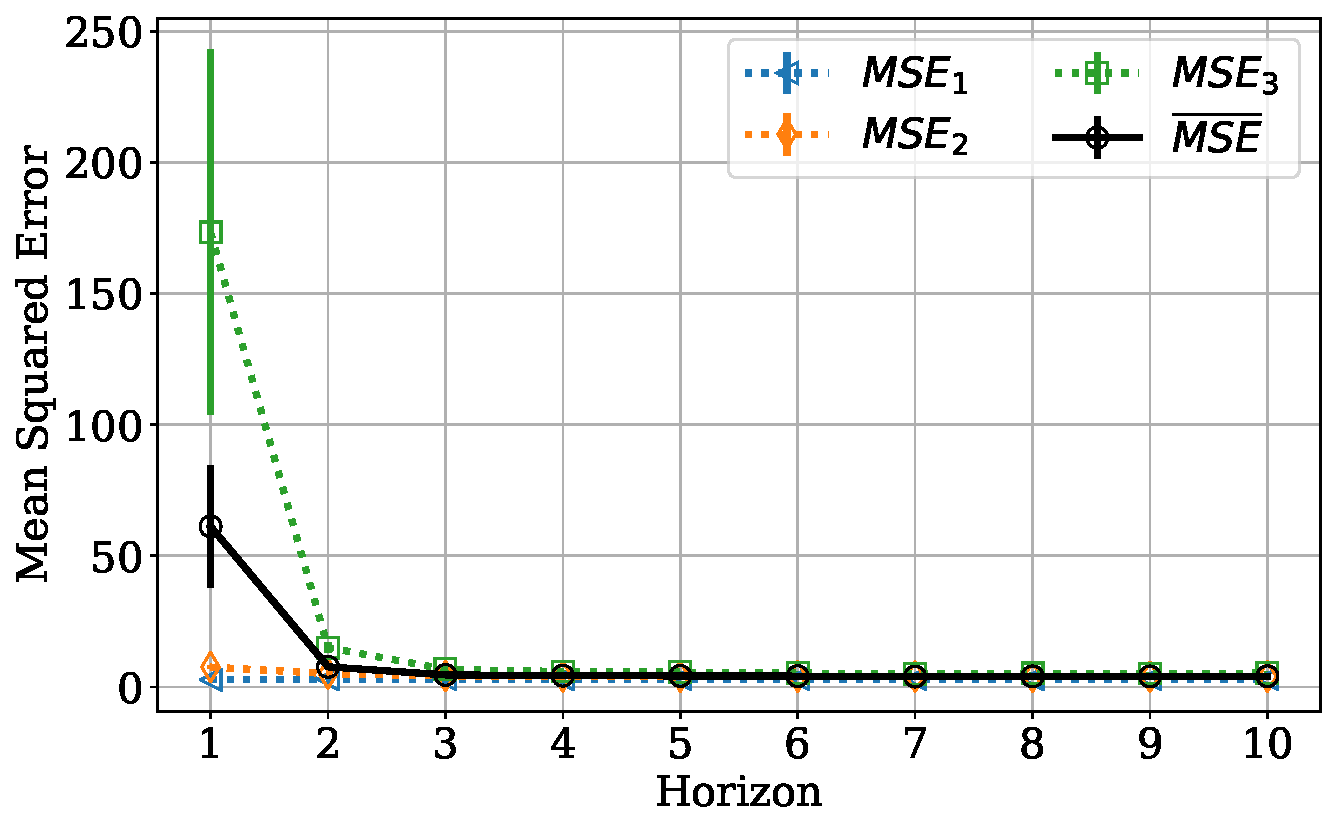
\includegraphics[width=\textwidth]{FHS2_MSE_against_H_separate}
    \caption{Scenario 3 with FHS}
  \end{subfigure}
  \hfill
  \begin{subfigure}[b]{0.49\textwidth}
    \centering
    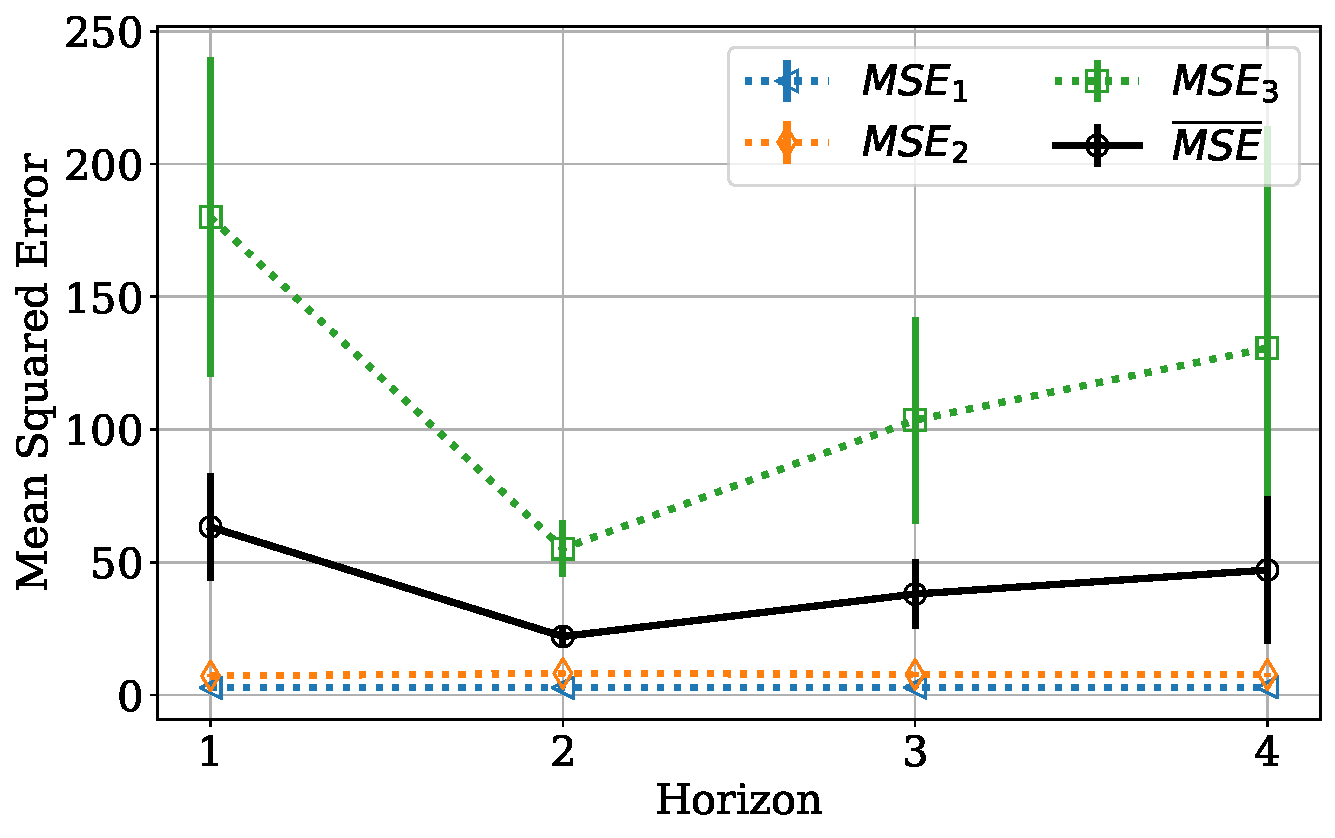
\includegraphics[width=\textwidth]{GES2_MSE_against_H_separate}
    \caption{Scenario 3 with GES}
  \end{subfigure}
  \caption{Scenario 2 \& 3: Average MSE vs. finite horizon $H$}
  \label{fig:MSEavg2}
\end{figure}

\subsection{Discussion}

It is evident that performance achieved by the proposed schedulers are
influenced by the length of burst errors. While FHS is relatively robust to
varying bursty channels, GES tends to show instable behavior. However, we can
observe the general trend that as the scheduler looks further in the future with
increasing $H$, it becomes more aware of potential high costs and adjusts
network share to prevent these.

One of the key design parameters for the proposed scheduling algorithm is the
selection of $H$. Fig.~\ref{fig:networkshare} visualizes the effect of selected
$H$ on the scheduling policy obtained from our proposed  FH scheduling scheme.
For any given finite horizon $H$ and number of control loops $N$, the size of
the underlying tree structure grows exponentially with $N\cdot H$. On the other
hand, a larger $H$ makes the scheduler more farsighted which may lead to an
improvement in performance. However, Fig.~\ref{fig:MSEavg} shows that the
expected performance gain it brings in terms of cost diminishes after a certain
$H$ value. Consequently, a finite $H$ can be chosen without losing any notable
performance. 

To get an idea on how scheduler complexity increases with $H$,
Tab.~\ref{tab:complexity} compares the average number of nodes in the root tree
during simulations (GES) to its base scheduler (FHS) and the worst-case (WC)
with sampling period $D_i=1$. We observe that being fully GE-aware incurs
substantial complexity, reflected in the average node count for WC and GES. This
is because GES takes independent GE channel transitions into account, while FHS
assumes a constant channel. We further notice the impact of constraining the
action set as in Eq.~\eqref{eq:admissibleactions} on the tree size. In our
implementation, the search space is reduced up to on average compared to the
worst-case scenario.

\begin{table}[htb]
  \begin{center}
  \begin{tabular}{|l|c|c|c|c|}
  \hline
  $H$ & 1 & 2 & 3 & 4 \\ 
  \hline \hline
  \textbf{GES} & 30.9 & $8.7\cdot10^2$ & $2.3\cdot10^4$ & $5.9\cdot10^5$ \\
  \textbf{FHS} & 4.6 & $17.6$ & $58.3$ & $1.9\cdot10^2$ \\
  \textbf{WC} & 33.0 & $1.1\cdot10^3$ & $3.4\cdot10^4$ & $1.1\cdot10^6$ \\
  \hline
  \end{tabular}
  \caption{Average node count of FHS and GES tree structures}
  \label{tab:complexity}
  \end{center}
\end{table}

Nevertheless, finding the global optimum by considering every possible network
outcome is not scalable, especially for NCS scenarios with Gilbert-Elliot
channels. During evaluation we stopped GES simulations at $H=4$ as runtime were
not feasible for subsequent horizons. To tackle scalability for the proposed
approach, a trade-off has to be found between complexity by increasing H and
complexity by decreasing H. In particular, the tree size has to be reduced
without neglecting possible GE channel transitions. Inspired by how reinforcement
learning copes with the \textit{exploration-exploitation dilemma}, a compromise
may be found with the following idea: The complete tree structure is built in a
FHS manner in order to constrain complexity. However, we are aware of the GE
channel by augmenting the branches at certain tree levels with transition
probabilities according to GES. One could uniformly decide at each level if a
channel transition should be considered, which makes such a scheduler
``explore'' for potential performance gains instead of exploiting thee
information it already has about the channel state.
